\documentclass[a4paper]{article}
\usepackage[english]{babel}
\usepackage[english]{inputenc}
\usepackage{t1enc}   %elválasztás!!!!

\usepackage{color}
\usepackage{amsmath}
\usepackage{amsfonts}
\usepackage{graphicx}
\usepackage{tikz}
\usepackage{pgfplots}
\usepackage{listings}
\usepackage{cancel}

\usetikzlibrary{arrows}
\graphicspath{ {images/} }

\author{Chan Pruksapha}

\let\oldref\ref
\renewcommand{\ref}[1]{(\oldref{#1})}

\begin{document}

\section*{Introduction: Markov Switching Auto-regressive}

In this section, we describe how markov-switching models arise in the context of modelling abrupt change in financial time series. In large part our explanation below is motivated by an exposition by Hamilton \cite{ham08}, although some modifications and extra content are added to suit our specific context.

Let begin by considering how we might describe the consequences of a dramatic change in the behavior of a single variable $y_t$. Suppose that the typical historical behavior could be described with a zero-mean first-order autoregression,

\begin{equation}\label{eq:phione}
y_t = \phi_1 y_{t-1} + \epsilon_t,
\end{equation}
$\epsilon_t \sim N(0,\sigma^2)$, which adequately describe the observed data up for $t = 1,2,\dots,t_0$.
Suppose that at date $t_0$ there was a significant change in the mean reverting rate of the series, so that we would instead wish to describe the data according to
\begin{equation}\label{eq:phitwo}
y_t = \phi_2 y_{t-1} + \epsilon_t 
\end{equation}
for $t = t_0+1, t_0+2, \dots$. On one hand, we could say that the series are governed by two different models \ref{eq:phione}, \ref{eq:phitwo} and there is a determistic shift in parameter shift after day $t_0$, but this is not satisfactory as a probability law that genereate data. The idea of regime switching model is that we, alternatively, encompass both models by a single, larger one
\begin{equation}
y_t = \phi_{s_t} y_{t-1} + \epsilon_t,
\end{equation}
in which we introducing a new variable $s_t$, which indicates whether or not we are in the first regime, or in the second regime, according to whether or not $t$ is before or after $t_0$. Specifically,
\begin{equation*}
s_t = 
\begin{cases}
1, & \text{ if } t\leq t_0,\\
2, & \text{ otherwise.}
\end{cases}
\end{equation*}


\begin{figure}[!h]
\centering
% The output from tikz()
% is imported here.
% Created by tikzDevice version 0.8.1 on 2015-06-29 01:14:31
% !TEX encoding = UTF-8 Unicode
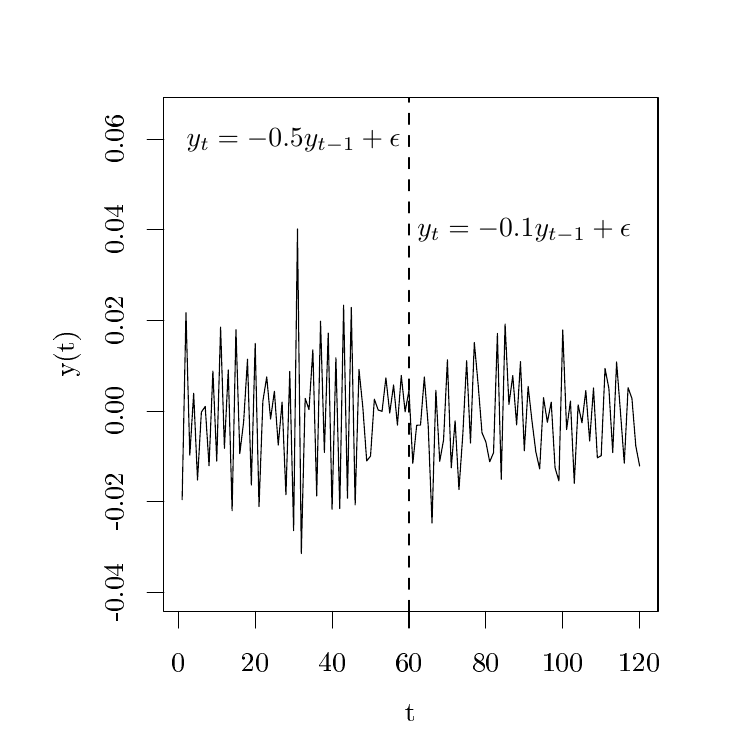
\begin{tikzpicture}[x=1pt,y=1pt]
\definecolor{fillColor}{RGB}{255,255,255}
\path[use as bounding box,fill=fillColor,fill opacity=0.00] (0,0) rectangle (252.94,252.94);
\begin{scope}
\path[clip] ( 49.20, 42.00) rectangle (227.75,227.75);
\definecolor{drawColor}{RGB}{0,0,0}

\path[draw=drawColor,line width= 0.4pt,line join=round,line cap=round] ( 55.81, 82.35) --
	( 57.20,149.96) --
	( 58.59, 98.44) --
	( 59.98,120.83) --
	( 61.37, 89.46) --
	( 62.76,114.00) --
	( 64.15,116.06) --
	( 65.54, 94.64) --
	( 66.93,128.85) --
	( 68.32, 96.29) --
	( 69.71,144.75) --
	( 71.09,100.94) --
	( 72.48,129.24) --
	( 73.87, 78.39) --
	( 75.26,143.81) --
	( 76.65, 99.06) --
	( 78.04,110.56) --
	( 79.43,133.12) --
	( 80.82, 87.65) --
	( 82.21,138.82) --
	( 83.60, 79.89) --
	( 84.99,118.00) --
	( 86.38,126.76) --
	( 87.77,111.52) --
	( 89.15,121.56) --
	( 90.54,102.08) --
	( 91.93,117.62) --
	( 93.32, 84.17) --
	( 94.71,128.75) --
	( 96.10, 71.21) --
	( 97.49,180.19) --
	( 98.88, 62.89) --
	(100.27,119.01) --
	(101.66,114.94) --
	(103.05,136.56) --
	(104.44, 83.72) --
	(105.83,146.88) --
	(107.21, 99.43) --
	(108.60,142.59) --
	(109.99, 78.91) --
	(111.38,133.65) --
	(112.77, 79.20) --
	(114.16,152.66) --
	(115.55, 82.90) --
	(116.94,151.86) --
	(118.33, 80.48) --
	(119.72,129.45) --
	(121.11,115.73) --
	(122.50, 96.38) --
	(123.89, 98.13) --
	(125.27,118.68) --
	(126.66,114.78) --
	(128.05,114.30) --
	(129.44,126.40) --
	(130.83,113.70) --
	(132.22,123.84) --
	(133.61,109.32) --
	(135.00,127.25) --
	(136.39,114.13) --
	(137.78,121.86) --
	(139.17, 95.52) --
	(140.56,109.27) --
	(141.95,109.34) --
	(143.33,126.72) --
	(144.72,109.25) --
	(146.11, 73.93) --
	(147.50,121.91) --
	(148.89, 96.23) --
	(150.28,103.98) --
	(151.67,132.94) --
	(153.06, 93.88) --
	(154.45,110.86) --
	(155.84, 86.06) --
	(157.23,105.86) --
	(158.62,132.60) --
	(160.01,102.81) --
	(161.39,139.17) --
	(162.78,123.91) --
	(164.17,106.54) --
	(165.56,103.28) --
	(166.95, 96.08) --
	(168.34, 99.35) --
	(169.73,142.45) --
	(171.12, 89.73) --
	(172.51,145.85) --
	(173.90,116.80) --
	(175.29,127.23) --
	(176.68,109.40) --
	(178.07,132.28) --
	(179.46,100.05) --
	(180.84,123.31) --
	(182.23,110.83) --
	(183.62, 99.68) --
	(185.01, 93.49) --
	(186.40,119.25) --
	(187.79,110.35) --
	(189.18,117.62) --
	(190.57, 93.88) --
	(191.96, 89.15) --
	(193.35,143.68) --
	(194.74,107.72) --
	(196.13,118.02) --
	(197.52, 88.31) --
	(198.90,116.64) --
	(200.29,110.19) --
	(201.68,121.81) --
	(203.07,103.57) --
	(204.46,122.74) --
	(205.85, 97.52) --
	(207.24, 98.27) --
	(208.63,129.79) --
	(210.02,122.54) --
	(211.41, 99.42) --
	(212.80,132.15) --
	(214.19,114.15) --
	(215.58, 95.57) --
	(216.96,122.85) --
	(218.35,118.93) --
	(219.74,101.80) --
	(221.13, 94.54);
\end{scope}
\begin{scope}
\path[clip] (  0.00,  0.00) rectangle (252.94,252.94);
\definecolor{drawColor}{RGB}{0,0,0}

\path[draw=drawColor,line width= 0.4pt,line join=round,line cap=round] ( 54.42, 42.00) -- (221.13, 42.00);

\path[draw=drawColor,line width= 0.4pt,line join=round,line cap=round] ( 54.42, 42.00) -- ( 54.42, 36.00);

\path[draw=drawColor,line width= 0.4pt,line join=round,line cap=round] ( 82.21, 42.00) -- ( 82.21, 36.00);

\path[draw=drawColor,line width= 0.4pt,line join=round,line cap=round] (109.99, 42.00) -- (109.99, 36.00);

\path[draw=drawColor,line width= 0.4pt,line join=round,line cap=round] (137.78, 42.00) -- (137.78, 36.00);

\path[draw=drawColor,line width= 0.4pt,line join=round,line cap=round] (165.56, 42.00) -- (165.56, 36.00);

\path[draw=drawColor,line width= 0.4pt,line join=round,line cap=round] (193.35, 42.00) -- (193.35, 36.00);

\path[draw=drawColor,line width= 0.4pt,line join=round,line cap=round] (221.13, 42.00) -- (221.13, 36.00);

\node[text=drawColor,anchor=base,inner sep=0pt, outer sep=0pt, scale=  1.00] at ( 54.42, 20.40) {0};

\node[text=drawColor,anchor=base,inner sep=0pt, outer sep=0pt, scale=  1.00] at ( 82.21, 20.40) {20};

\node[text=drawColor,anchor=base,inner sep=0pt, outer sep=0pt, scale=  1.00] at (109.99, 20.40) {40};

\node[text=drawColor,anchor=base,inner sep=0pt, outer sep=0pt, scale=  1.00] at (137.78, 20.40) {60};

\node[text=drawColor,anchor=base,inner sep=0pt, outer sep=0pt, scale=  1.00] at (165.56, 20.40) {80};

\node[text=drawColor,anchor=base,inner sep=0pt, outer sep=0pt, scale=  1.00] at (193.35, 20.40) {100};

\node[text=drawColor,anchor=base,inner sep=0pt, outer sep=0pt, scale=  1.00] at (221.13, 20.40) {120};

\path[draw=drawColor,line width= 0.4pt,line join=round,line cap=round] ( 49.20, 48.88) -- ( 49.20,212.68);

\path[draw=drawColor,line width= 0.4pt,line join=round,line cap=round] ( 49.20, 48.88) -- ( 43.20, 48.88);

\path[draw=drawColor,line width= 0.4pt,line join=round,line cap=round] ( 49.20, 81.64) -- ( 43.20, 81.64);

\path[draw=drawColor,line width= 0.4pt,line join=round,line cap=round] ( 49.20,114.40) -- ( 43.20,114.40);

\path[draw=drawColor,line width= 0.4pt,line join=round,line cap=round] ( 49.20,147.16) -- ( 43.20,147.16);

\path[draw=drawColor,line width= 0.4pt,line join=round,line cap=round] ( 49.20,179.92) -- ( 43.20,179.92);

\path[draw=drawColor,line width= 0.4pt,line join=round,line cap=round] ( 49.20,212.68) -- ( 43.20,212.68);

\node[text=drawColor,rotate= 90.00,anchor=base,inner sep=0pt, outer sep=0pt, scale=  1.00] at ( 34.80, 48.88) {-0.04};

\node[text=drawColor,rotate= 90.00,anchor=base,inner sep=0pt, outer sep=0pt, scale=  1.00] at ( 34.80, 81.64) {-0.02};

\node[text=drawColor,rotate= 90.00,anchor=base,inner sep=0pt, outer sep=0pt, scale=  1.00] at ( 34.80,114.40) {0.00};

\node[text=drawColor,rotate= 90.00,anchor=base,inner sep=0pt, outer sep=0pt, scale=  1.00] at ( 34.80,147.16) {0.02};

\node[text=drawColor,rotate= 90.00,anchor=base,inner sep=0pt, outer sep=0pt, scale=  1.00] at ( 34.80,179.92) {0.04};

\node[text=drawColor,rotate= 90.00,anchor=base,inner sep=0pt, outer sep=0pt, scale=  1.00] at ( 34.80,212.68) {0.06};

\path[draw=drawColor,line width= 0.4pt,line join=round,line cap=round] ( 49.20, 42.00) --
	(227.75, 42.00) --
	(227.75,227.75) --
	( 49.20,227.75) --
	( 49.20, 42.00);
\end{scope}
\begin{scope}
\path[clip] (  0.00,  0.00) rectangle (252.94,252.94);
\definecolor{drawColor}{RGB}{0,0,0}

\node[text=drawColor,anchor=base,inner sep=0pt, outer sep=0pt, scale=  1.00] at (138.47,  2.40) {t};

\node[text=drawColor,rotate= 90.00,anchor=base,inner sep=0pt, outer sep=0pt, scale=  1.00] at ( 16.80,134.87) {y(t)};
\end{scope}
\begin{scope}
\path[clip] ( 49.20, 42.00) rectangle (227.75,227.75);
\definecolor{drawColor}{RGB}{0,0,0}

\node[text=drawColor,anchor=base,inner sep=0pt, outer sep=0pt, scale=  1.00] at ( 96.10,210.18) {$y_t = -0.5 y_{t-1} + \epsilon$};

\node[text=drawColor,anchor=base,inner sep=0pt, outer sep=0pt, scale=  1.00] at (179.46,177.42) {$y_t = -0.1 y_{t-1} + \epsilon$};

\path[draw=drawColor,line width= 0.4pt,dash pattern=on 4pt off 4pt ,line join=round,line cap=round] (137.78, 42.00) -- (137.78,227.75);
\end{scope}
\end{tikzpicture}

\caption{Simple Example}
\end{figure}


\begin{figure}[!h]
\centering
% The output from tikz()
% is imported here.
% Created by tikzDevice version 0.8.1 on 2015-06-29 01:14:32
% !TEX encoding = UTF-8 Unicode
\begin{tikzpicture}[x=1pt,y=1pt]
\definecolor{fillColor}{RGB}{255,255,255}
\path[use as bounding box,fill=fillColor,fill opacity=0.00] (0,0) rectangle (252.94,252.94);
\begin{scope}
\path[clip] ( 49.20, 61.20) rectangle (227.75,203.75);
\definecolor{drawColor}{RGB}{0,0,0}

\path[draw=drawColor,line width= 0.4pt,line join=round,line cap=round] ( 55.81, 66.48) --
	( 57.20, 66.48) --
	( 58.59, 66.48) --
	( 59.98, 66.48) --
	( 61.37, 66.48) --
	( 62.76, 66.48) --
	( 64.15, 66.48) --
	( 65.54, 66.48) --
	( 66.93, 66.48) --
	( 68.32, 66.48) --
	( 69.71, 66.48) --
	( 71.09, 66.48) --
	( 72.48, 66.48) --
	( 73.87, 66.48) --
	( 75.26, 66.48) --
	( 76.65, 66.48) --
	( 78.04, 66.48) --
	( 79.43, 66.48) --
	( 80.82, 66.48) --
	( 82.21, 66.48) --
	( 83.60, 66.48) --
	( 84.99, 66.48) --
	( 86.38, 66.48) --
	( 87.77, 66.48) --
	( 89.15, 66.48) --
	( 90.54, 66.48) --
	( 91.93, 66.48) --
	( 93.32, 66.48) --
	( 94.71, 66.48) --
	( 96.10, 66.48) --
	( 97.49, 66.48) --
	( 98.88, 66.48) --
	(100.27, 66.48) --
	(101.66, 66.48) --
	(103.05, 66.48) --
	(104.44, 66.48) --
	(105.83, 66.48) --
	(107.21, 66.48) --
	(108.60, 66.48) --
	(109.99, 66.48) --
	(111.38, 66.48) --
	(112.77, 66.48) --
	(114.16, 66.48) --
	(115.55, 66.48) --
	(116.94, 66.48) --
	(118.33, 66.48) --
	(119.72, 66.48) --
	(121.11, 66.48) --
	(122.50, 66.48) --
	(123.89, 66.48) --
	(125.27, 66.48) --
	(126.66, 66.48) --
	(128.05, 66.48) --
	(129.44, 66.48) --
	(130.83, 66.48) --
	(132.22, 66.48) --
	(133.61, 66.48) --
	(135.00, 66.48) --
	(136.39, 66.48) --
	(137.78, 66.48) --
	(139.17,198.47) --
	(140.56,198.47) --
	(141.95,198.47) --
	(143.33,198.47) --
	(144.72,198.47) --
	(146.11,198.47) --
	(147.50,198.47) --
	(148.89,198.47) --
	(150.28,198.47) --
	(151.67,198.47) --
	(153.06,198.47) --
	(154.45,198.47) --
	(155.84,198.47) --
	(157.23,198.47) --
	(158.62,198.47) --
	(160.01,198.47) --
	(161.39,198.47) --
	(162.78,198.47) --
	(164.17,198.47) --
	(165.56,198.47) --
	(166.95,198.47) --
	(168.34,198.47) --
	(169.73,198.47) --
	(171.12,198.47) --
	(172.51,198.47) --
	(173.90,198.47) --
	(175.29,198.47) --
	(176.68,198.47) --
	(178.07,198.47) --
	(179.46,198.47) --
	(180.84,198.47) --
	(182.23,198.47) --
	(183.62,198.47) --
	(185.01,198.47) --
	(186.40,198.47) --
	(187.79,198.47) --
	(189.18,198.47) --
	(190.57,198.47) --
	(191.96,198.47) --
	(193.35,198.47) --
	(194.74,198.47) --
	(196.13,198.47) --
	(197.52,198.47) --
	(198.90,198.47) --
	(200.29,198.47) --
	(201.68,198.47) --
	(203.07,198.47) --
	(204.46,198.47) --
	(205.85,198.47) --
	(207.24,198.47) --
	(208.63,198.47) --
	(210.02,198.47) --
	(211.41,198.47) --
	(212.80,198.47) --
	(214.19,198.47) --
	(215.58,198.47) --
	(216.96,198.47) --
	(218.35,198.47) --
	(219.74,198.47) --
	(221.13,198.47);
\end{scope}
\begin{scope}
\path[clip] (  0.00,  0.00) rectangle (252.94,252.94);
\definecolor{drawColor}{RGB}{0,0,0}

\path[draw=drawColor,line width= 0.4pt,line join=round,line cap=round] ( 54.42, 61.20) -- (221.13, 61.20);

\path[draw=drawColor,line width= 0.4pt,line join=round,line cap=round] ( 54.42, 61.20) -- ( 54.42, 55.20);

\path[draw=drawColor,line width= 0.4pt,line join=round,line cap=round] ( 82.21, 61.20) -- ( 82.21, 55.20);

\path[draw=drawColor,line width= 0.4pt,line join=round,line cap=round] (109.99, 61.20) -- (109.99, 55.20);

\path[draw=drawColor,line width= 0.4pt,line join=round,line cap=round] (137.78, 61.20) -- (137.78, 55.20);

\path[draw=drawColor,line width= 0.4pt,line join=round,line cap=round] (165.56, 61.20) -- (165.56, 55.20);

\path[draw=drawColor,line width= 0.4pt,line join=round,line cap=round] (193.35, 61.20) -- (193.35, 55.20);

\path[draw=drawColor,line width= 0.4pt,line join=round,line cap=round] (221.13, 61.20) -- (221.13, 55.20);

\node[text=drawColor,anchor=base,inner sep=0pt, outer sep=0pt, scale=  1.00] at ( 54.42, 39.60) {0};

\node[text=drawColor,anchor=base,inner sep=0pt, outer sep=0pt, scale=  1.00] at ( 82.21, 39.60) {20};

\node[text=drawColor,anchor=base,inner sep=0pt, outer sep=0pt, scale=  1.00] at (109.99, 39.60) {40};

\node[text=drawColor,anchor=base,inner sep=0pt, outer sep=0pt, scale=  1.00] at (137.78, 39.60) {60};

\node[text=drawColor,anchor=base,inner sep=0pt, outer sep=0pt, scale=  1.00] at (165.56, 39.60) {80};

\node[text=drawColor,anchor=base,inner sep=0pt, outer sep=0pt, scale=  1.00] at (193.35, 39.60) {100};

\node[text=drawColor,anchor=base,inner sep=0pt, outer sep=0pt, scale=  1.00] at (221.13, 39.60) {120};

\path[draw=drawColor,line width= 0.4pt,line join=round,line cap=round] ( 49.20, 61.20) --
	(227.75, 61.20) --
	(227.75,203.75) --
	( 49.20,203.75) --
	( 49.20, 61.20);
\end{scope}
\begin{scope}
\path[clip] (  0.00,  0.00) rectangle (252.94,252.94);
\definecolor{drawColor}{RGB}{0,0,0}

\node[text=drawColor,anchor=base,inner sep=0pt, outer sep=0pt, scale=  1.00] at (138.47, 15.60) {t};

\node[text=drawColor,rotate= 90.00,anchor=base,inner sep=0pt, outer sep=0pt, scale=  1.00] at ( 10.80,132.47) {s(t)};
\end{scope}
\begin{scope}
\path[clip] (  0.00,  0.00) rectangle (252.94,252.94);
\definecolor{drawColor}{RGB}{0,0,0}

\path[draw=drawColor,line width= 0.4pt,line join=round,line cap=round] ( 49.20, 66.48) -- ( 49.20,198.47);

\path[draw=drawColor,line width= 0.4pt,line join=round,line cap=round] ( 49.20, 66.48) -- ( 43.20, 66.48);

\path[draw=drawColor,line width= 0.4pt,line join=round,line cap=round] ( 49.20,198.47) -- ( 43.20,198.47);

\node[text=drawColor,rotate= 90.00,anchor=base,inner sep=0pt, outer sep=0pt, scale=  1.00] at ( 34.80, 66.48) {1};

\node[text=drawColor,rotate= 90.00,anchor=base,inner sep=0pt, outer sep=0pt, scale=  1.00] at ( 34.80,198.47) {2};
\end{scope}
\end{tikzpicture}

\caption{Simple Example}
\end{figure}

A complete description of the probability law governing the observed data would then require a probabilistic model of what caused the change from $s_t = 1 \text{ to } s_t = 2$. The simplest such specification is that $s_t$ is the realization of a two-state Markov chain with

\begin{equation} \label{eq:tranprob}
\mathbb{P}(s_t = i | s_{t-1} = j, s_{t-2}, \dots, y_{t-1}, y_{t-2}, \dots) = \mathbb{P}(s_t = i | s_{t-1} = j) := p_{ij}.
\end{equation}

The specification in \ref{eq:tranprob} assumes that the probability of a change in regime depends on the past only through the value of the most recent regime. Although there are some excellent discussions (e.g., \cite{dieb94}, \cite{fil94}) about time-varying transitional probability, of which the dependency of past observation $y_{t-1}, y_{t-2} , \dots$ are maintained as in LHS., it is found in most applications that regime switching models work well under markov assumption.

\section*{Formal Definitions}

\begin{equation}
y_t = c_{s_t} + \sum_{i=1}^L \phi_i^{s_t} y + \epsilon_t
\end{equation}

\begin{equation}
A=
\begin{bmatrix}
    p_{11}       & p_{12} & p_{13} & \dots & p_{1S} \\
    p_{21}       & p_{22} & x_{23} & \dots & p_{2S} \\
    \hdotsfor{5} \\
    p_{S1}       & p_{S2} & p_{S3} & \dots & p_{SS}
\end{bmatrix}
\end{equation}

\section*{Learning and Inferences}

\subsection*{EM algorithm}
 To do.
\subsection*{Forward Filtering}

Next, we discuss how do we infer which regime our time series $y_t$ is falling in on a particular day $t$. Equations \ref{eq:fwdfilt1}, \ref{eq:fwdfilt2} and \ref{eq:fwdfilt3} below are the derivation of probability that the regime variable $s_t$ equals to regime $i$, conditioning on all the past observations $y_t, y_{t-1}, \dots$ that are available up to day $t$.

\begin{equation}\label{eq:fwdfilt1}
\mathbb{P}(s_t = i | y_t, y_{t-1}, \dots) = \frac{ \mathbb{P}(y_t | s_t = i, y_{t-1}, y_{t-2}, \dots) \mathbb{P}(s_t = i | y_{t-1}, \dots) } { \mathbb{P}(y_t | y_{t-1}, \dots)}
\end{equation}
\begin{equation}\label{eq:fwdfilt2}
\mathbb{P}(s_t = i | y_{t-1}, \dots) = \sum_{j=1}^{S} \mathbb{P}(s_t = i | s_{t-1} = j, y_{t-1}, \dots) \mathbb{P}(s_{t-1} = j | y_{t-1}, \dots) 
\end{equation}

By applying markov assumption\footnote{$p_{ij}=\mathbb{P}(s_t = i | s_{t-1} = j) = \mathbb{P}(s_t = i | s_{t-1} = j, \cancel{y_{t-1}}, \dots).$} equations \ref{eq:fwdfilt1} and \ref{eq:fwdfilt2} become

\begin{equation} \label{eq:fwdfilt3}
\mathbb{P}(s_t = i | y_t, \dots) \text{\;$\propto$\footnotemark\;} \mathbb{P}(y_t | s_t = i, y_{t-1}, \dots) \sum_{j=1}^{S} p_{ij} \mathbb{P}(s_{t-1} = j | y_{t-1}, \dots). 
\end{equation}
\footnotetext{The normalizing constant, ${\mathbb{P}(y_t | y_{t-1}, \dots) = \sum_{i=1}^{2} \mathbb{P}(y_t | s_t = i, y_{t-1}, y_{t-2}, \dots) \mathbb{P}(s_t = i | y_{t-1},} \dots)$, is actually the summation of the RHS. of \ref{eq:fwdfilt3} over $i\in\{1,\dots,S\}$.}

\section*{Training}

\begin{figure}[!h]
\centering
\input{images/firstTrained.eps}
\caption{Jan 2002 - Decempber 2009}
\end{figure}




\begin{thebibliography}{1}
\bibitem{ham08} Hamilton, J.D. (2008). Regime-switching models. In: S. Durlauf and L. Blume (eds.), New Palgrave dictionary of economics, 2nd edition. Palgrave McMillan Ltd.
\bibitem{dieb94} Diebold, F.X., J.H. Lee, and G.C. Weinbach. Regime Switching with Time-Varying Transition Probabilities. In: C. Hargreaves, ed., Nonstationary Time Series Analysis and Cointegration. Oxford, UK: Oxford University Press, 1994, pp. 283-302.
\bibitem{fil94} Filardo, A.J., 1994, Business cycle phases and their transitional dynamics. Journal of Business and Economic Statistics 12, 299 308. 
\end{thebibliography}

\end{document}



